\documentclass[10pt,handout,english]{beamer}
\usepackage[utf8]{inputenc} 
%{vietnam}
\usepackage[scheme=plain]{ctex} %{ctex, hyperref}
% \usepackage[T1]{fontenc}
\usepackage{xcolor}
\usepackage{enumitem}
\usepackage{graphicx} % For including images
\usepackage{caption} 
\usepackage{tikz}
\usepackage{algorithm,algorithmic}
% \usepackage[backend=bibtex,style=authoryear]{biblatex}

%---------Theme----------
\usetheme{Madrid}
\definecolor{blockcolor}{RGB}{60, 155, 45}
\setbeamercolor{block title}{bg=blue!30, fg=black} % Màu nền và màu chữ của tiêu đề block
\setbeamercolor{block body}{bg=blue!10} % Màu nền của nội dung block
\setbeamercolor{block title alerted}{bg=blockcolor, fg=white} % Màu nền và màu chữ của tiêu đề block khi sử dụng block alert
\setbeamercolor{block body alerted}{bg=green!10} % Màu nền của nội dung block khi sử dụng block alert (đổi sang màu xám)




% other packages
\usepackage{amsmath, amsthm, amssymb, latexsym, amscd, amsfonts, enumerate}
\usepackage{multicol,booktabs,calligra}
\usepackage{graphicx,pstricks,listings,stackengine}
\usepackage{extarrows}

\author{Ho Thuy Tram, Thai Gia Huy}
\title{Lempel-Ziv-Welch (LZW) Compression}
\subtitle{Data Structures and Algorithms}
\institute{University of Science - VNU HCMC}
\date{\empty}
\usepackage{BeamerSieuCapVjpPro}

% defs
\def\cmd#1{\texttt{\color{red}\footnotesize $\backslash$#1}}
\def\env#1{\texttt{\color{blue}\footnotesize #1}}
\definecolor{deepblue}{rgb}{0,0,0.5}
\definecolor{deepred}{rgb}{0.6,0,0}
\definecolor{deepgreen}{rgb}{0,0.5,0}
\definecolor{halfgray}{gray}{0.55}

\lstset{
    basicstyle=\ttfamily\small,
    keywordstyle=\bfseries\color{deepblue},
    emphstyle=\ttfamily\color{deepred},    % Custom highlighting style
    stringstyle=\color{deepgreen},
    numbers=left,
    numberstyle=\small\color{halfgray},
    rulesepcolor=\color{red!20!green!20!blue!20},
    frame=shadowbox,
}

\setbeamertemplate{itemize item}{\color{red}\raise0.2ex\hbox{\large\textbullet}}


% \usepackage[backend=biber,style=numeric-comp,sorting=none]{biblatex}
% \usepackage{filecontents}

% \begin{filecontents*}{ref.bib}
% @ARTICLE{2,
%   author={Ziv, J. and Lempel, A.},
%   journal={IEEE Transactions on Information Theory}, 
%   title={Compression of individual sequences via variable-rate coding}, 
%   year={1978},
%   volume={24},
%   number={5},
%   pages={530-536},
%   keywords={},
%   doi={10.1109/TIT.1978.1055934}}

% @article{3,
%   title={A technique for high-performance data compression},
%   author={Welch, Terry A.},
%   journal={Computer},
%   volume={17},
%   number={06},
%   pages={8--19},
%   year={1984},
%   publisher={IEEE Computer Society}
% }

% @article{1,
%   title={A universal algorithm for sequential data compression},
%   author={Jacob Ziv and Abraham Lempel},
%   journal={IEEE Trans. Inf. Theory},
%   year={1977},
%   volume={23},
%   pages={337-343},
%   url={https://api.semanticscholar.org/CorpusID:9267632}
% }
% \end{filecontents*}

% \addbibresource{ref.bib}



\begin{document}

% \kaishu
\setmainfont{Times New Roman}
\begin{frame}
% \begin{center}
% \begin{tikzpicture}[remember picture, overlay]
%     % VNU logo
%     \node[opacity=0.2,inner sep=0pt] at (0, 0) {
\includegraphics[width=1\textwidth]{Figures/0. General/VNU_gray.png}};
    
%     % HCMUS logo
%     \node[inner sep=0pt] (logo) at (-3, 0) {
\includegraphics[width=.55\textwidth]{Figures/0. General/hcmus.png}};
    
%     % FIT
%     \node[text width=0.5\textwidth, right=of logo] (title) {
\includegraphics[width=.6\textwidth]{Figures/0. General/fit.png}};
    
%     % Red line
%     \draw[line width=1mm, Tue-red] ($(logo.east) + (0.5, 1.3)$) -- ($(logo.east) + (0.5, -1.3)$);
% \end{tikzpicture}
% \end{center}
    \titlepage
    % \begin{figure}[htpb]
    %     \begin{center}
    %         
\includegraphics[width=0.2\linewidth]{pic/HCMUS - logo.pdf}
    %     \end{center}
    % \end{figure}
\end{frame}

\begin{frame}
    \tableofcontents[sectionstyle=show,subsectionstyle=show/shaded/hide,subsubsectionstyle=show/shaded/hide]
\end{frame}

\section{Introduction}
\subsection{Basic introduction to Data Compression }
\begin{frame}{Basic introduction to data compression}
    \textbf{\large{What is Data Compression, at first?}}
    
    \vspace{0.5pt}
    
    \begin{itemize} [label=\textcolor{purple}{$\bullet$}]
        \item  A process of reducing the amount of data "represented by bits" needed for the storage or transmission.
        \vspace{0.2pt}
        \item Important in storing information digitally on computer disks and in transmitting it over communication channels.
        \vspace{0.2pt}
        \item Since the size of data increases over time, compression methods enable efficient data transfer at lower bandwidth by utilizing payload.
    \end{itemize}
\end{frame}

\subsection{Historical Background of LZW Compression}

\begin{frame}{Historical Background}
    \begin{minipage}{0.49\textwidth}
        \centering
        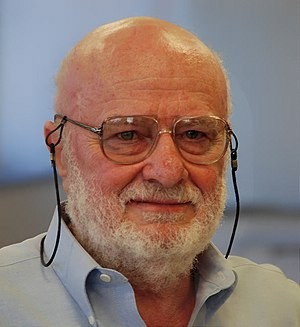
\includegraphics[width=0.6\textwidth, height=0.7\textwidth]{pic/lempel.jpg}
        \captionof{figure}{Abraham Lempel}
    \end{minipage}%
    \hfill
    \begin{minipage}{0.49\textwidth}
        \centering
        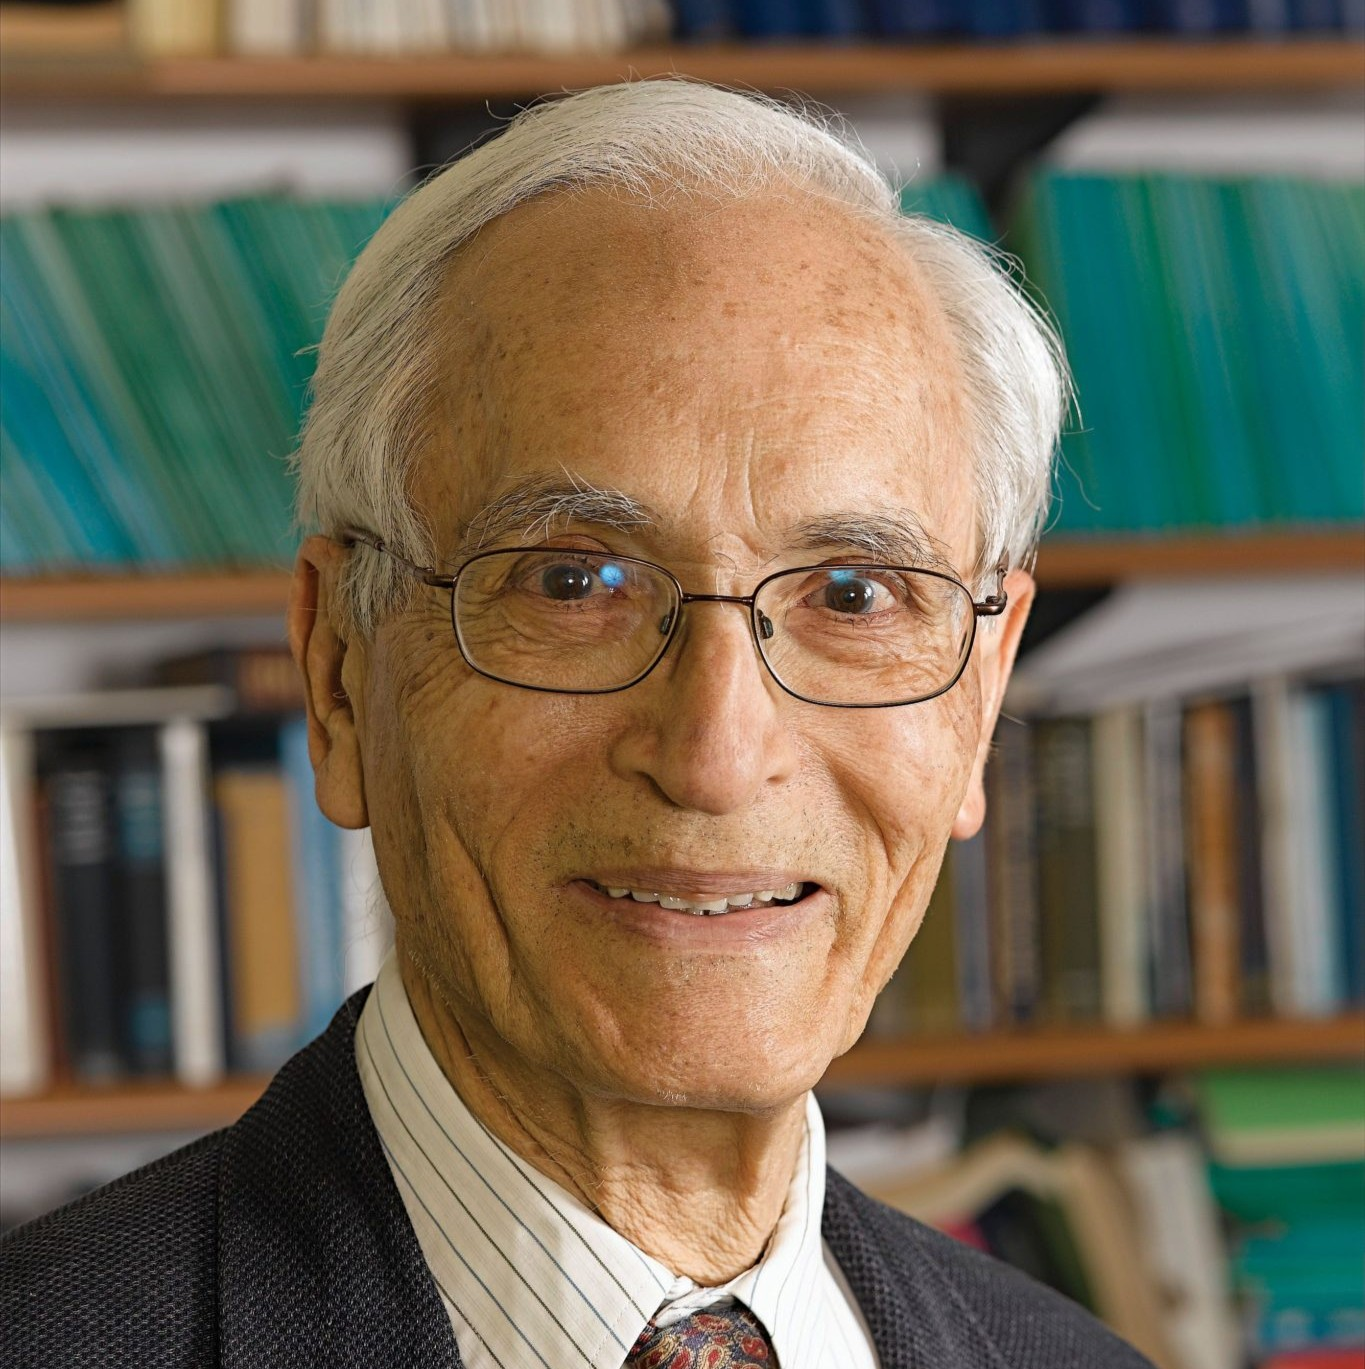
\includegraphics[width=0.6\textwidth, height=0.7\textwidth]{pic/Ziv.jpeg}
        \captionof{figure}{Jacob Ziv}
    \end{minipage}
    
    \begin{itemize} [label=\textcolor{purple}{$\bullet$}]
        \item  Upon the pioneering work of Abraham Lempel and Jacob Ziv on LZ7, LZ78, published in \textit{IEEE Transactions on Information Theory}.
    \end{itemize}
\end{frame}

\begin{frame}{Historical Background}
    \begin{minipage}{0.49\textwidth}
        \centering
        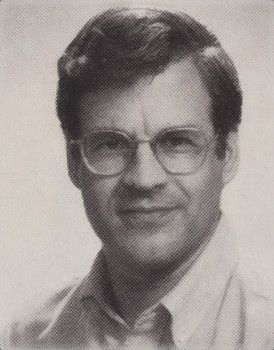
\includegraphics[width=0.6\textwidth, height=0.7\textwidth]{pic/welch.jpg}
        \captionof{figure}{Abraham Lempel}
    \end{minipage}%
    \hfill
    \begin{minipage}{0.49\textwidth}
        \centering
        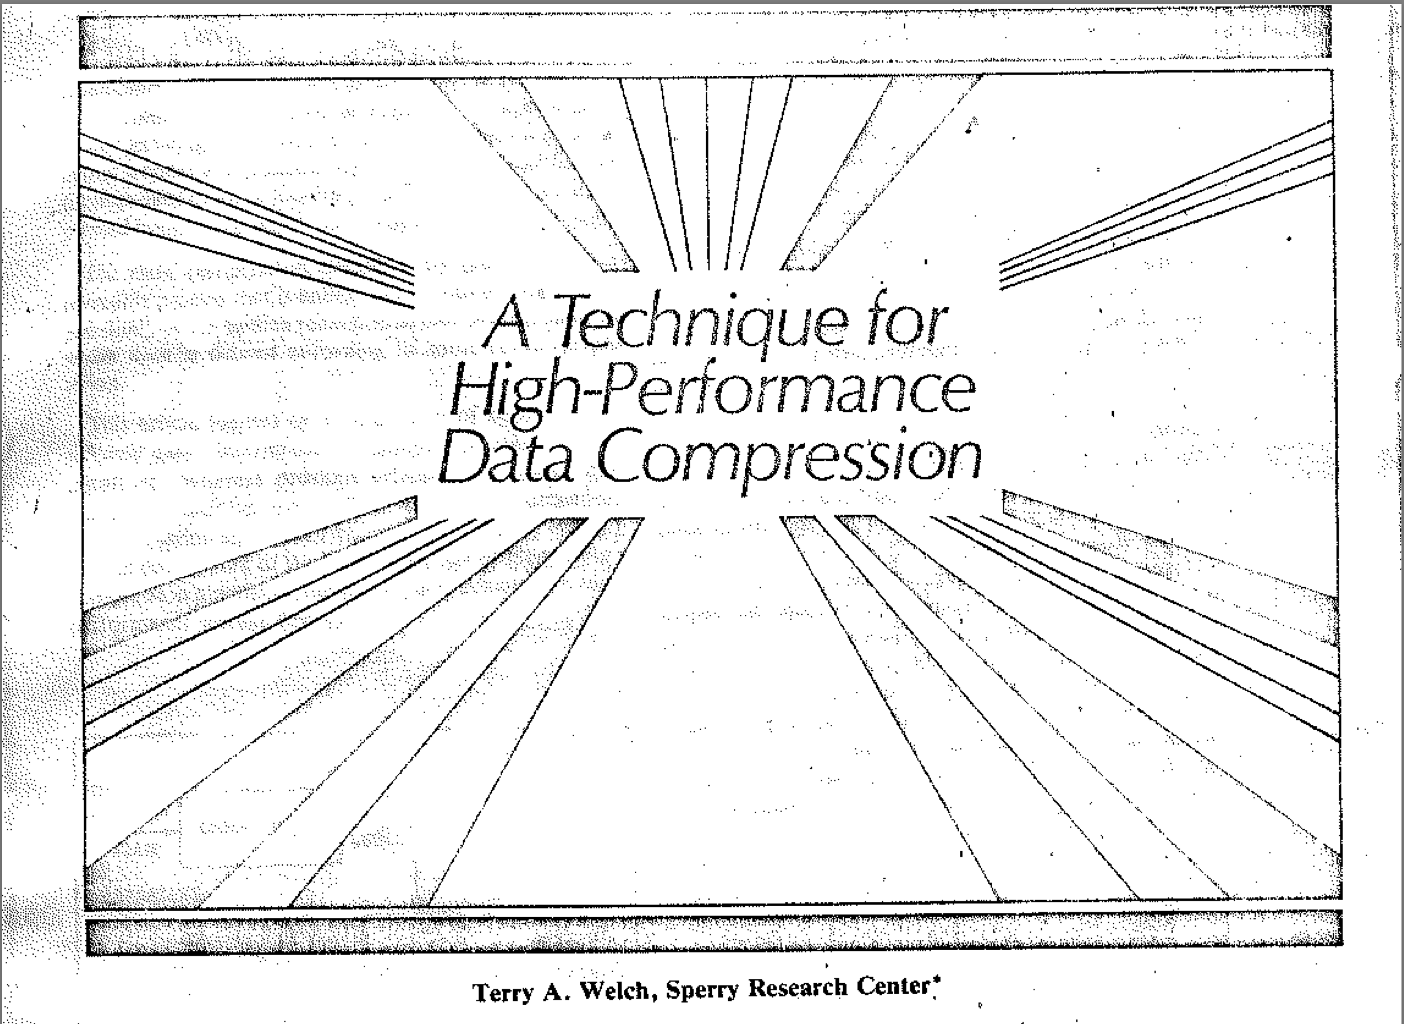
\includegraphics[width=0.6\textwidth, height=0.7\textwidth]{pic/paper1984.png}
        \captionof{figure}{Lempel-Ziv-Welch paper}
    \end{minipage}
 
    \begin{itemize} [label=\textcolor{purple}{$\bullet$}]
        \item  Terry Welch further refined the algorithm to improve its efficiency and adaptiveness, leading to his 1984 article, "A Technique for High-Performance Data Compression", published in \textit{Computer}.
    \end{itemize}
\end{frame}


\subsection{Applications of LZW Compression}

\begin{frame}{Applications}
    \centering
    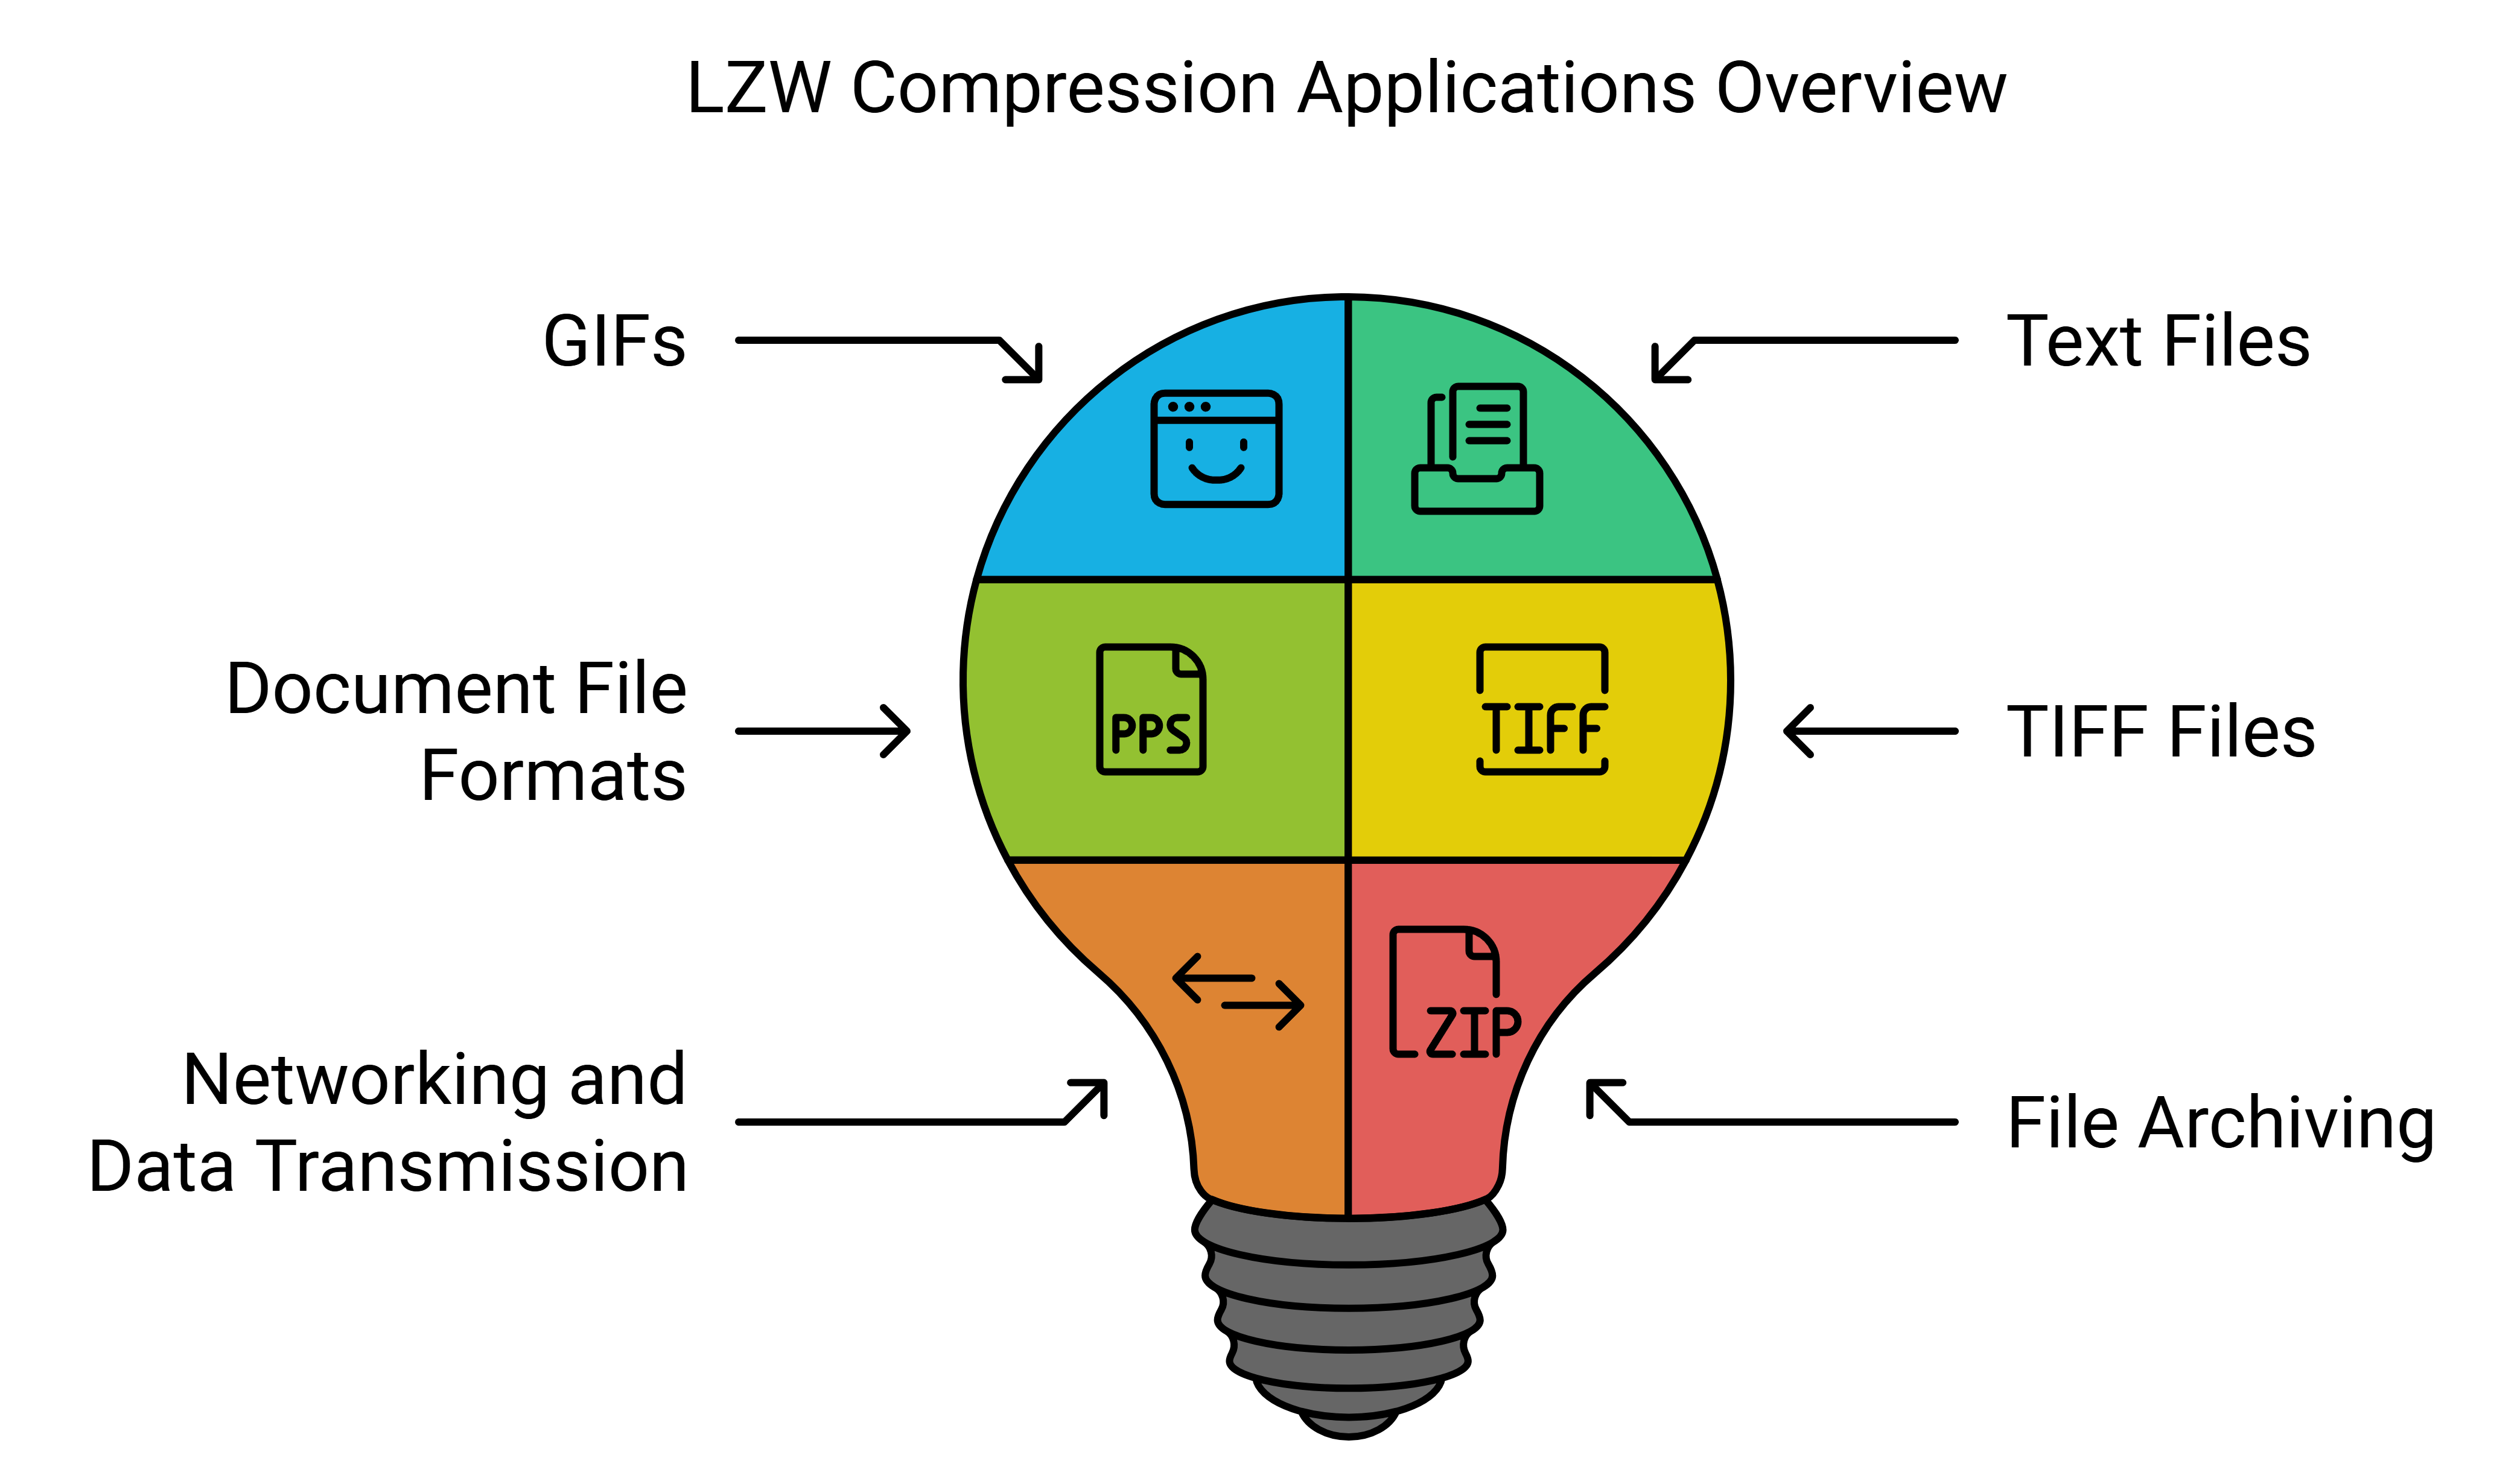
\includegraphics[width=0.7\textwidth]{pic/application.png}
    \vspace{0.2cm}
\end{frame}

\section{Understanding the Algorithm}
\subsection{Key Concepts and Mechanisms}

\begin{frame}{Key Concepts and Mechanisms (1)}
    Lossless Dictionary-based method
    \begin{itemize}[label=\textcolor{purple}{$\bullet$}]
        \item To "memorize" the substrings of characters that occurred before in the text.
        \vspace{0.2pt}
        \item  Uses the indices of the place in the dictionary where the substring is stored.
    \end{itemize}

    "Greedy" parsing algorithm 
    \begin{itemize}[label=\textcolor{purple}{$\bullet$}]
        \item The text is looped over exactly once, during this parsing, the longest recognized substring is saved to the encoded results.
        \vspace{0.2pt}
        \item  "The current substring + the next character" is added to the dictionary.
    \end{itemize}
    
\end{frame}

\begin{frame}{Key Concepts and Mechanisms (2)}
    \begin{itemize}[label=\textcolor{purple}{$\bullet$}]
        \item No dictionary transmission which reduces transmission overhead. The dynamic dictionary is created by both compressor and decompressor with a small dictionary.
        \item Relies heavily on the nature of the input data. Does not attempt to optimally select strings by making use of probability estimation.
        \item Therefore, its effectiveness is less than optimal but creates great usability by the simplicity of the algorithm.
    \end{itemize}
\end{frame}

\subsection{Compression Phase with Examples}
\begin{frame}{Compression Phase}
    \begin{figure}
        \centering
        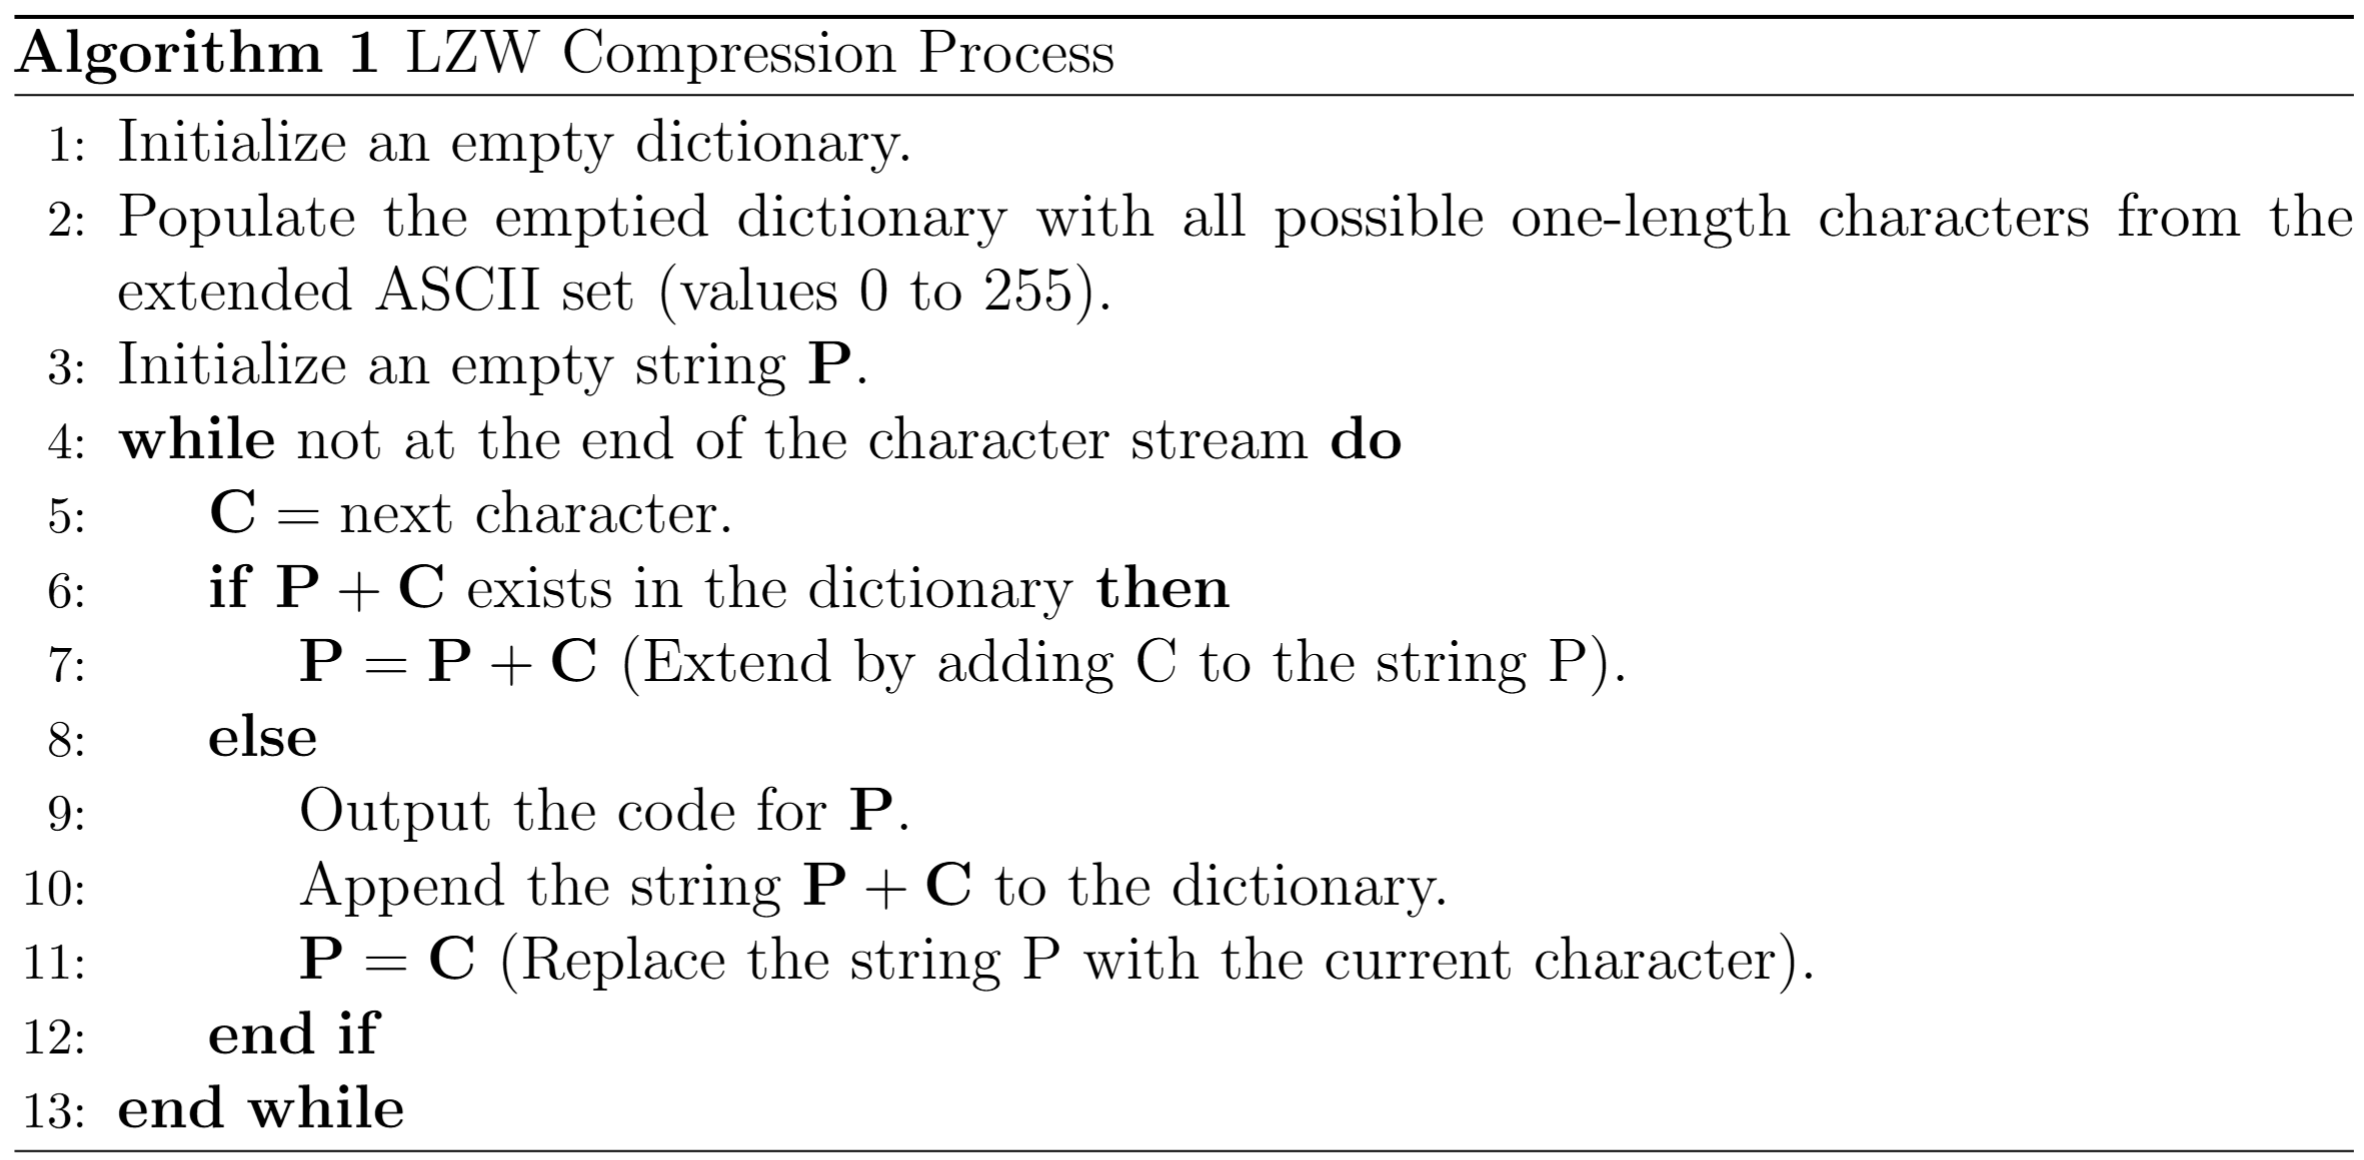
\includegraphics[width=0.9\textwidth]{pic/pseudo_compress.png}
    \end{figure}
    
\end{frame}

\begin{frame}{Compression Process with Step by Step}
    \begin{figure}
        \centering
        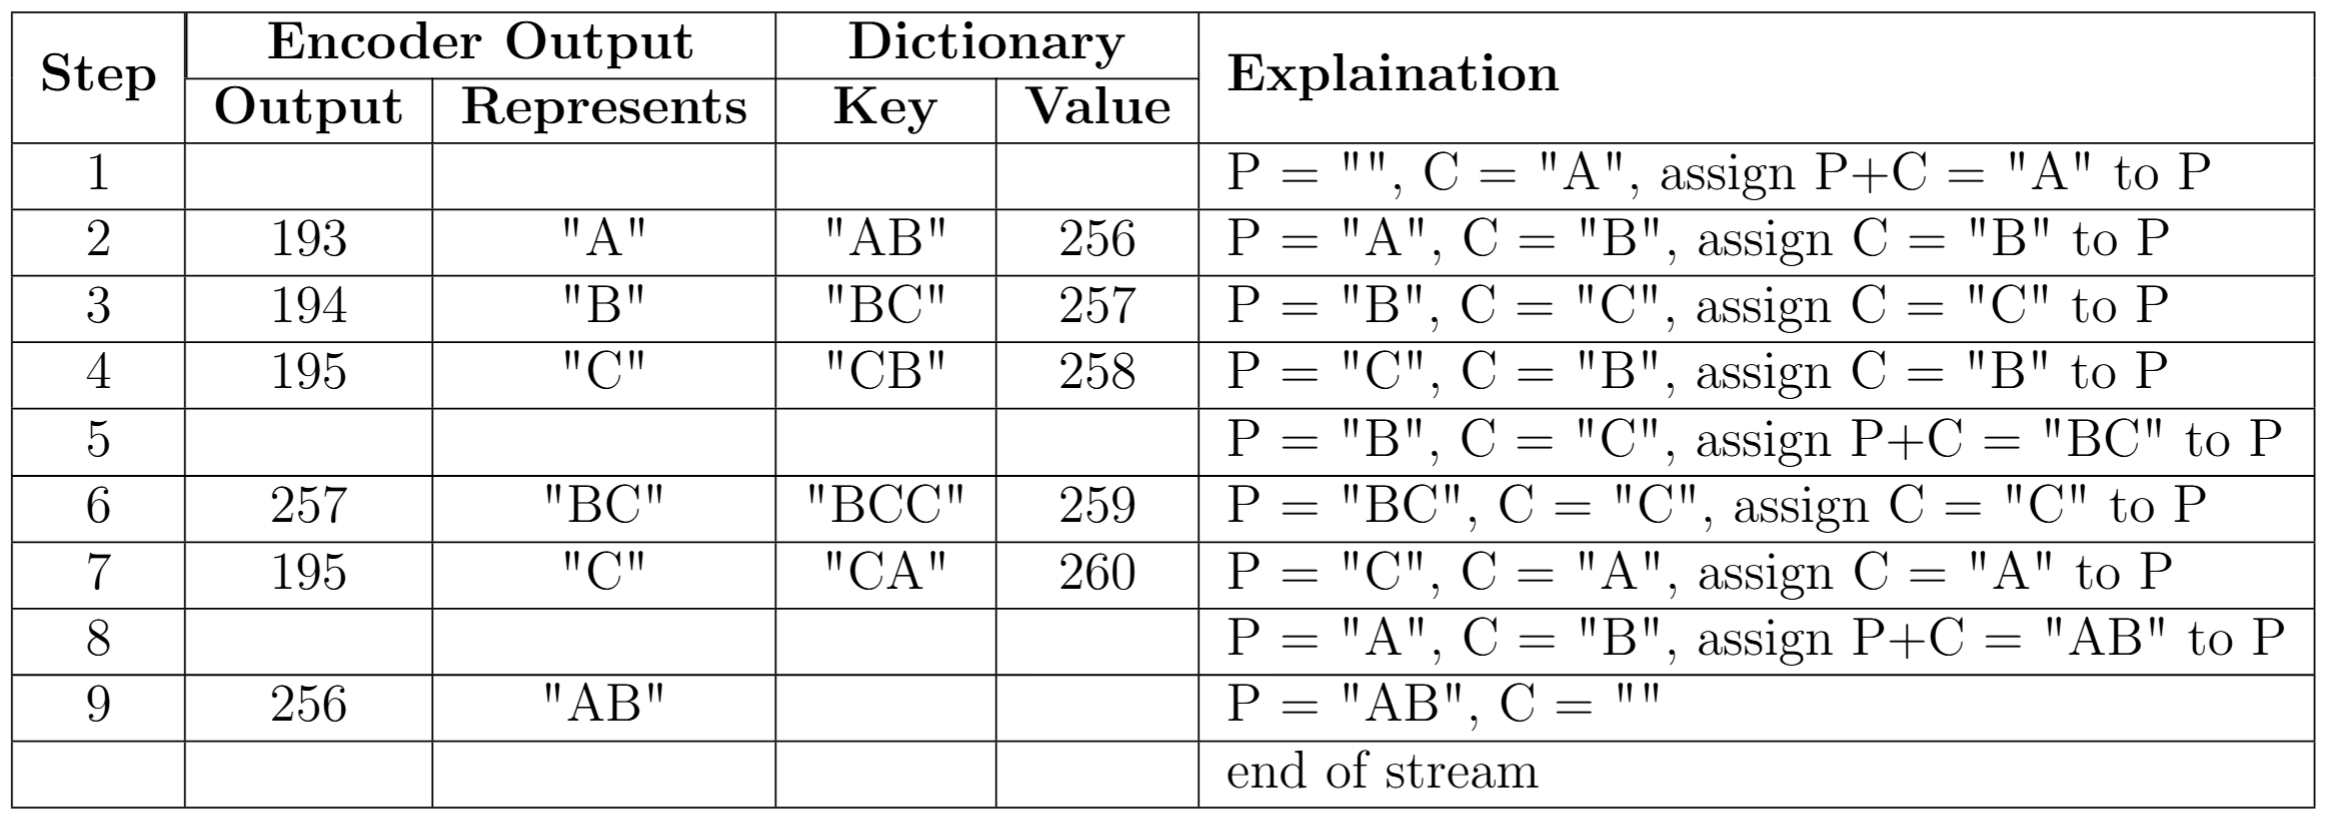
\includegraphics[width=0.9\textwidth]{pic/example_compress.png}
    \end{figure}
\end{frame}

\subsection{Decompression Phase with Examples}
\begin{frame}{Decompression Phase}
    \begin{figure}
        \centering
        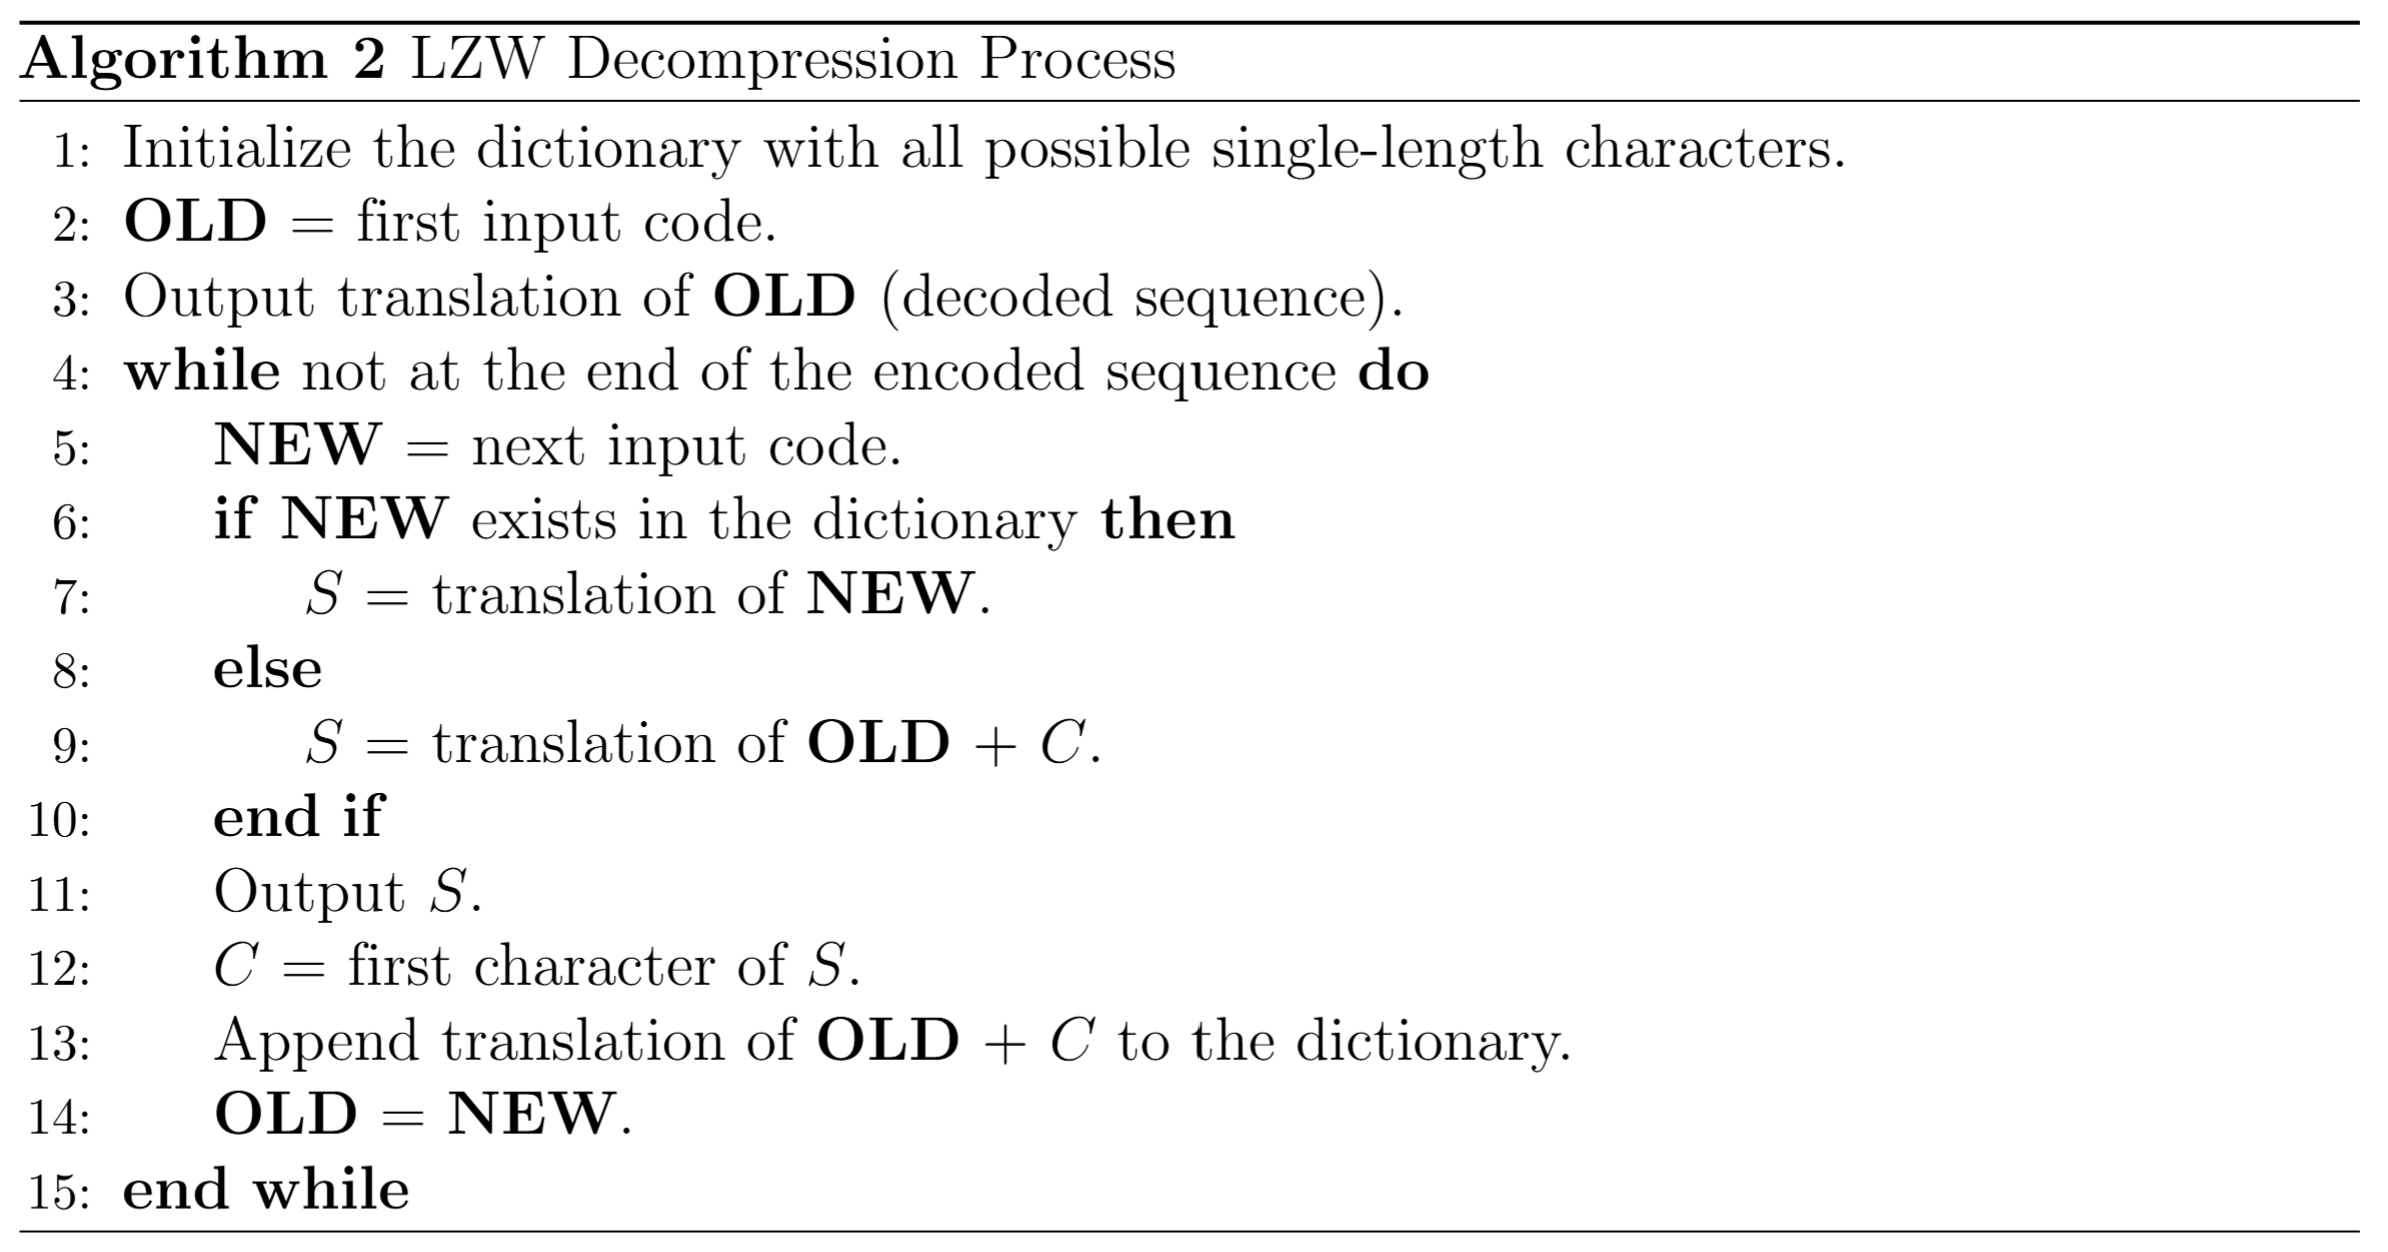
\includegraphics[width=0.9\textwidth]{pic/pseudo_decompress.png}
    \end{figure}
\end{frame}

\begin{frame}{Deompression Process with Step by Step}
    \begin{figure}
        \centering
        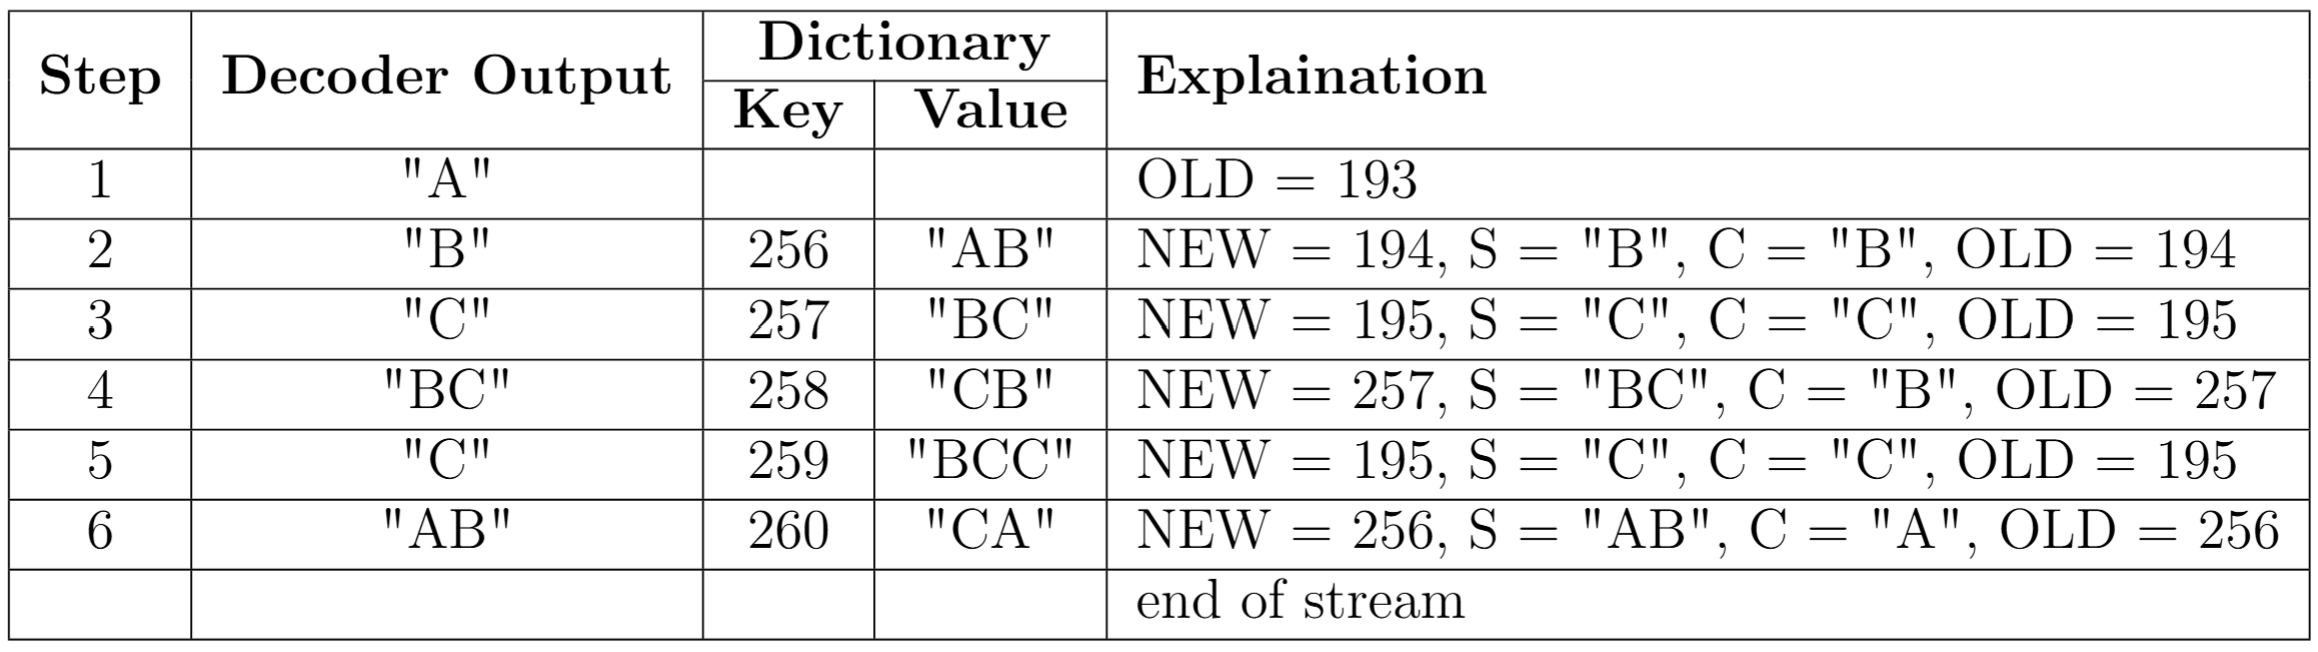
\includegraphics[width=0.9\textwidth]{pic/example_decompress.png}
    \end{figure}
\end{frame}

\newpage

\section{Performance Analysis}
\subsection{Compression Ratios}

\begin{frame}{Compression Ratios}
    \begin{table}[h!]
    \centering
    \begin{tabular}{|l|c|}
    \hline
    \textbf{Data Type}               & \textbf{Compression Ratio} \\ \hline
    English Text                     & 1.8                        \\ \hline
    Cobol Files                      & 2 to 6                     \\ \hline
    Floating Point Arrays            & 1.0                        \\ \hline
    Formatted Scientific Data        & 2.1                        \\ \hline
    System Log Data                  & 2.6                        \\ \hline
    Program Source Code              & 2.3                        \\ \hline
    Object Code                      & 1.5                        \\ \hline
    \end{tabular}
    \label{tab:compression_results}
    \end{table}
\end{frame}

\subsection{Time Complexity}

\begin{frame}{Best Case for English Text}
    \begin{figure}[ht]
    \centering
    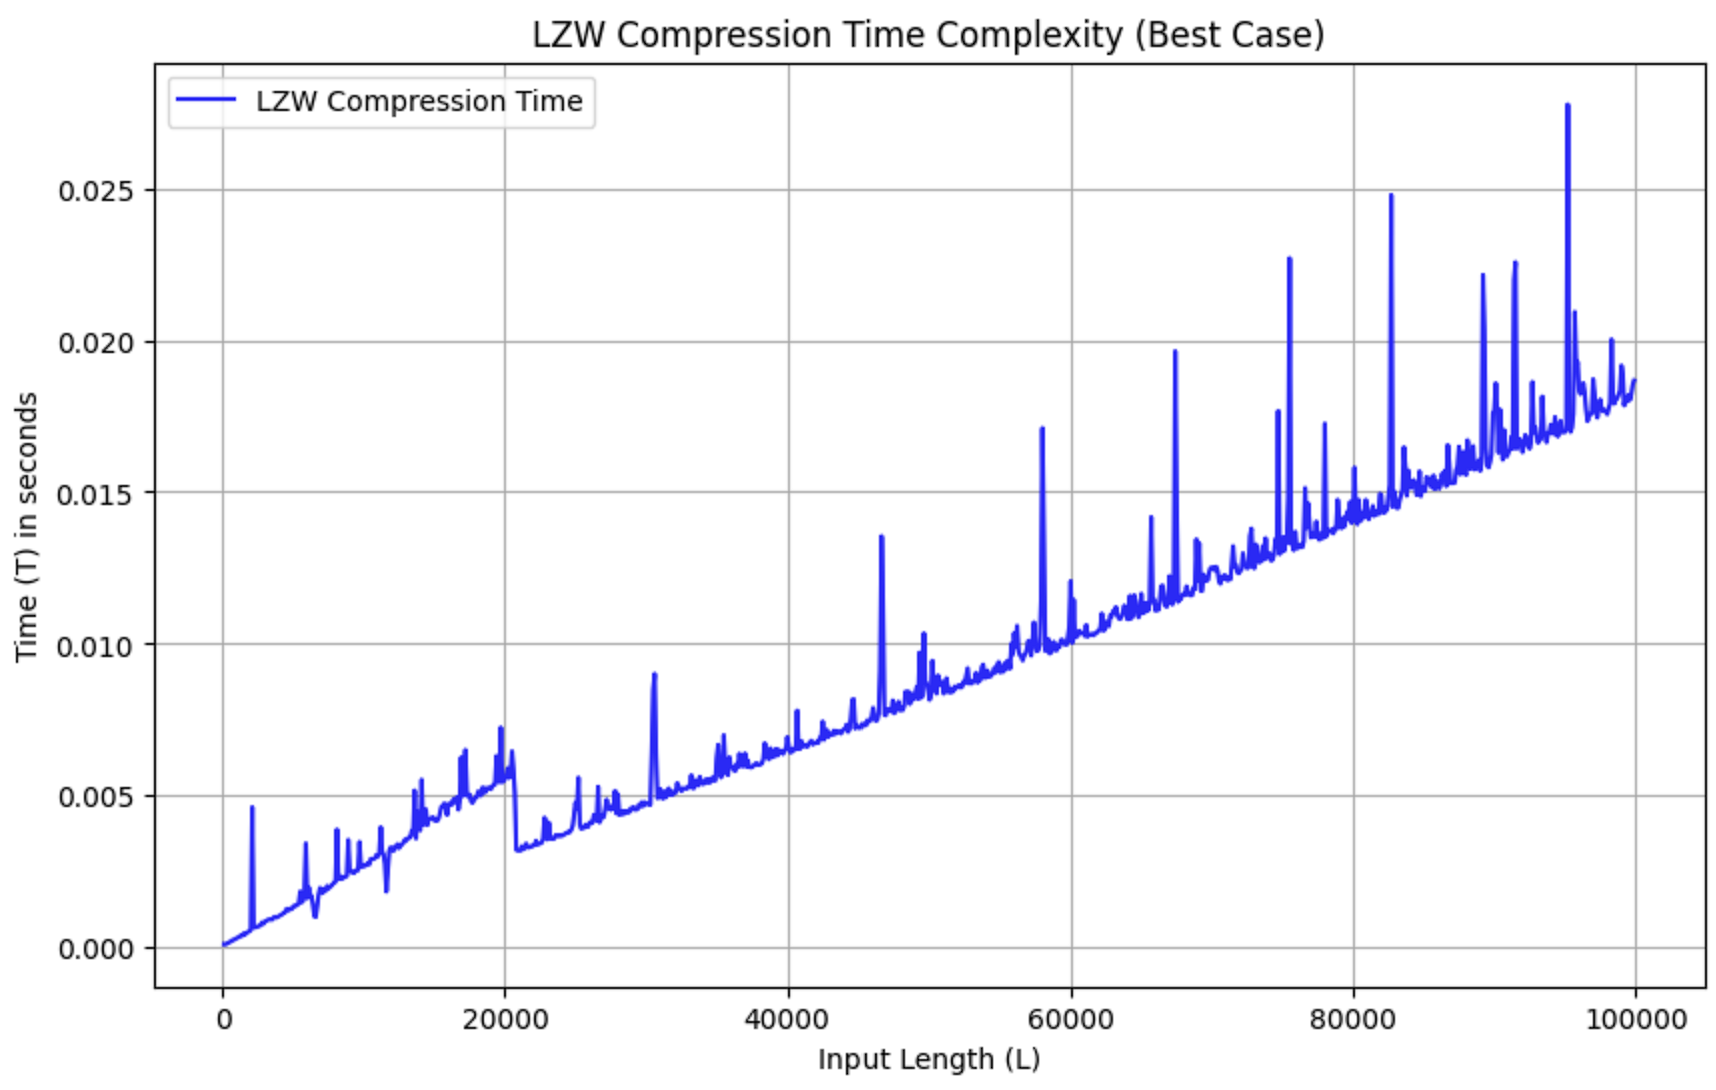
\includegraphics[width=0.5\linewidth]{pic/best_case.png}
    \caption{LZW Compression Runtime in Best Case}
    \label{fig:bestcase}
    \end{figure}
\end{frame}

\begin{frame}{Best Case for English Text}
    \begin{figure}[ht]
    \centering
    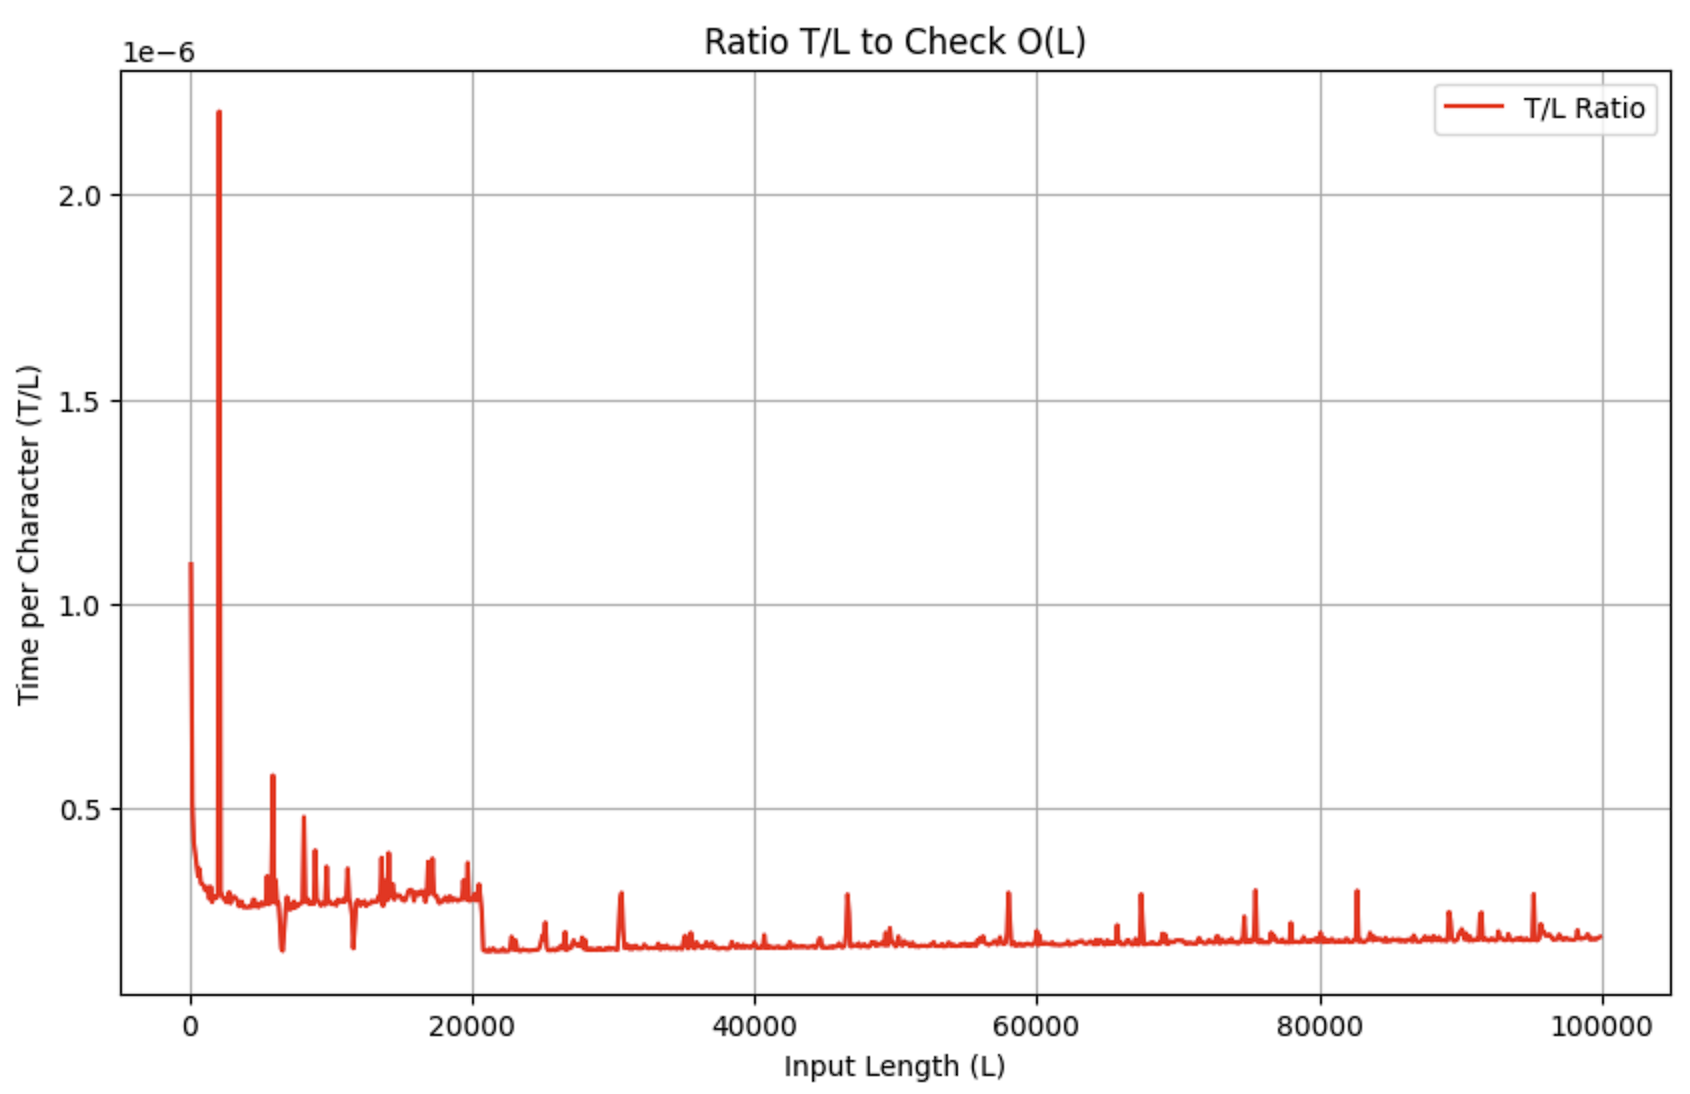
\includegraphics[width=0.5\linewidth]{pic/bestcase_prove.png}
    \caption{Best Case: $T = \mathcal{O}(L)$}
\end{figure}
\end{frame}

\begin{frame}{Worst Case for English Text}
    \begin{figure}[ht]
    \centering
    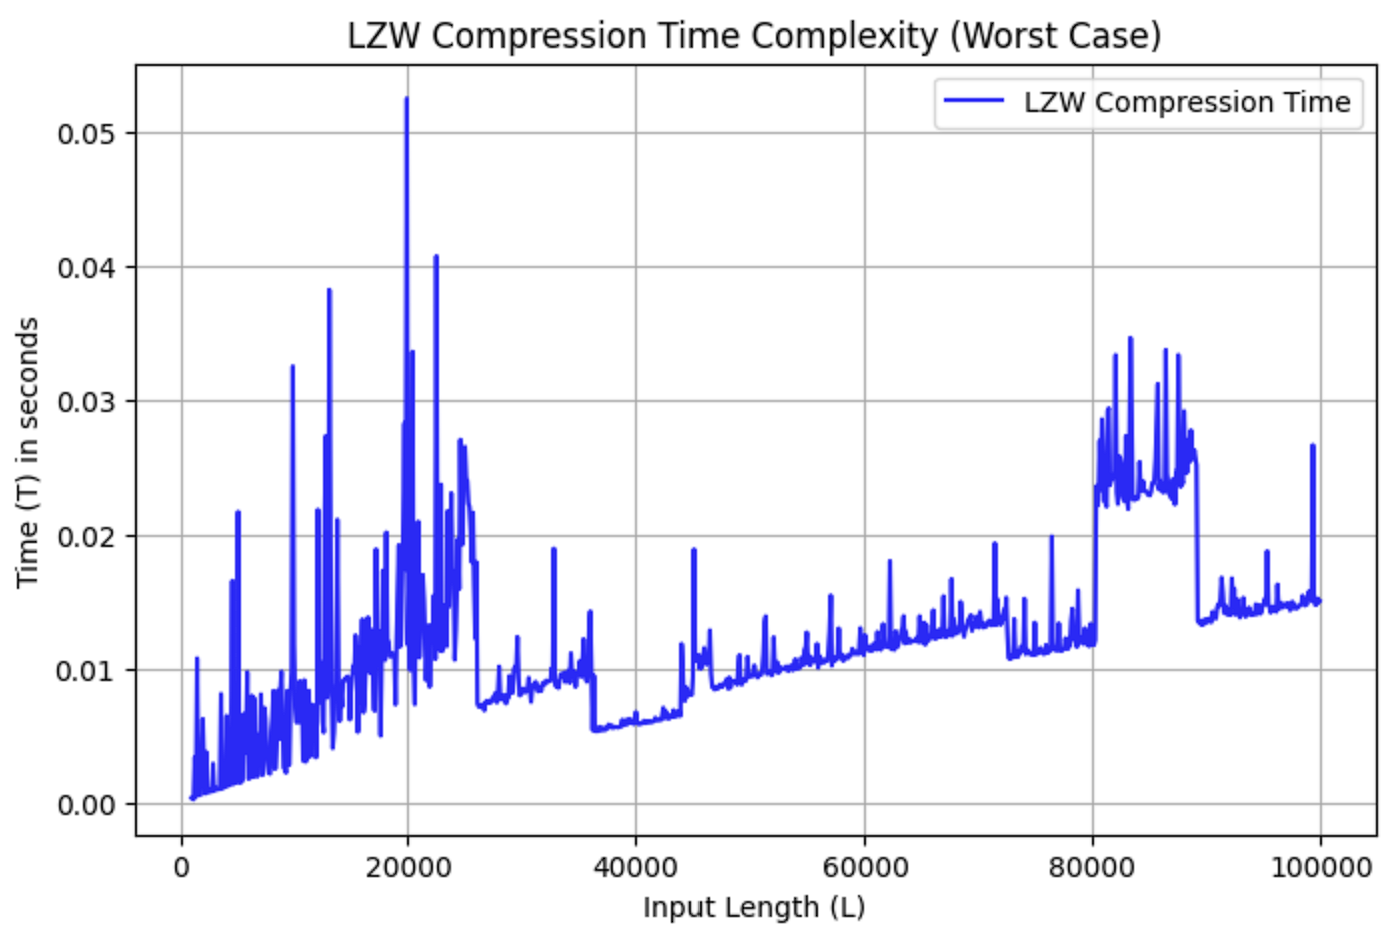
\includegraphics[width=0.5\linewidth]{pic/worst_case.png}
    \caption{LZW Compression Runtime in Worst Case}
    \label{fig:bestcase}
    \end{figure}
\end{frame}

\begin{frame}{Worst Case for English Text}
    \begin{figure}[ht]
    \centering
    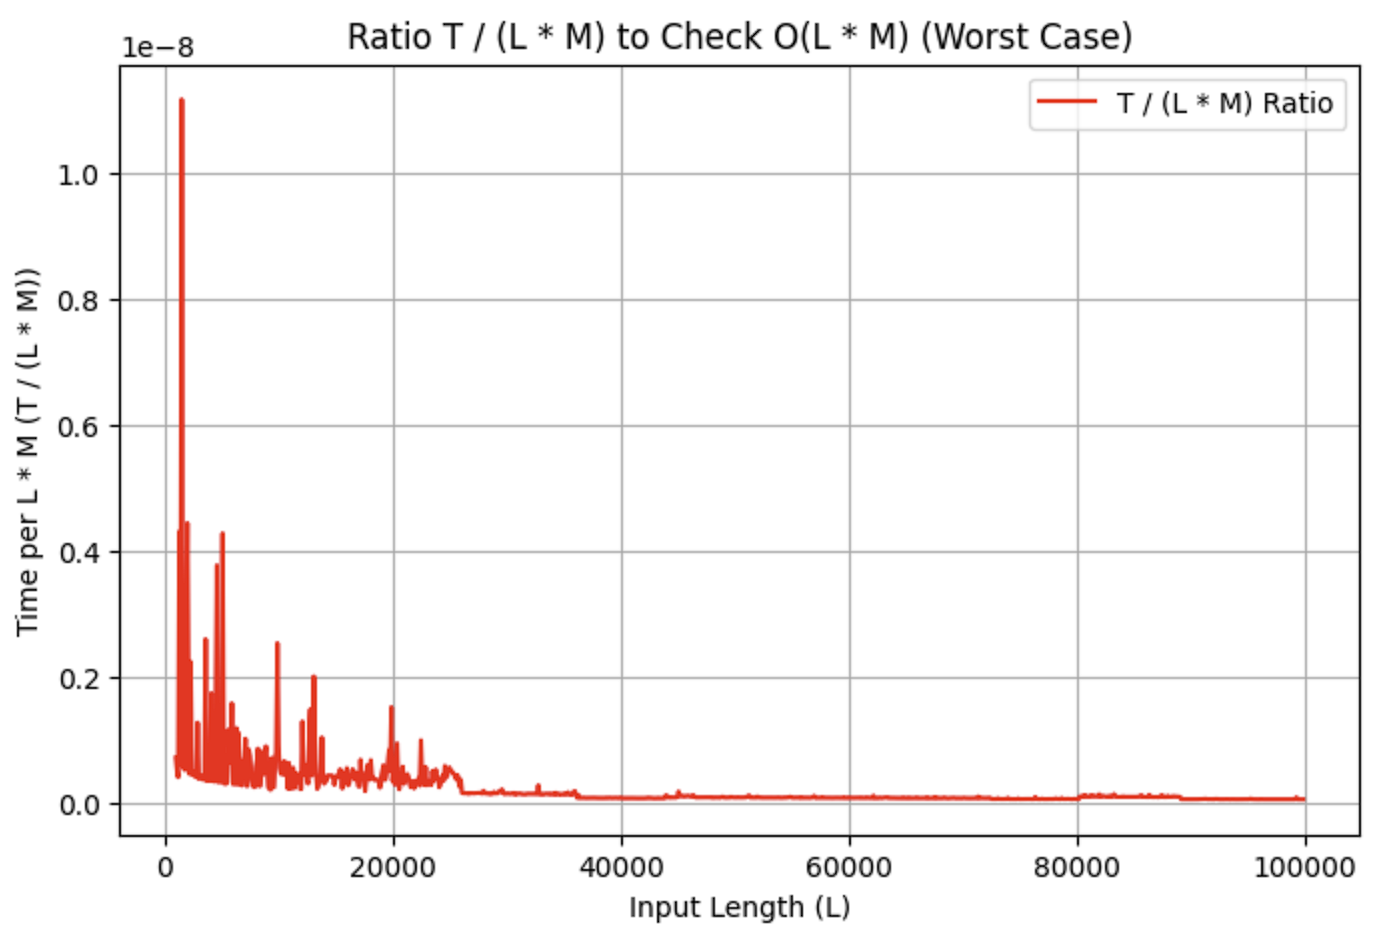
\includegraphics[width=0.5\linewidth]{pic/worstcase_prove.png}
    \caption{Best Case: $T = \mathcal{O}(L \cdot M)$}
    \label{fig:enter-label}
\end{figure}
\end{frame}

\newpage

\section{Overview of LZW-Related Algorithms}

\subsection{LZ77}

\begin{frame}{LZ77}
    \begin{itemize}
        \item \textbf{Concept}: Uses a \textit{sliding window} to find matches between the lookahead buffer and previous data.
        \item \textbf{Compression Output}: A triplet \((\text{offset}, \text{length}, \text{symbol})\).
        % \item Offset: Position of match in the sliding window.
        % \item Length: Number of matched characters.
        % \item Symbol: First unmatched character.
    \end{itemize}
    \begin{table}[h!]
        \centering
        \begin{tabular}{|p{3.5cm}|p{5cm}|}
        \hline
        \textbf{Strengths} & \textbf{Weaknesses}    \\ \hline
        Efficient for localized patterns & Less efficient for globally repetitive data \\ \hline
        Simple implementation & Limited range due to sliding window \\ \hline
        \end{tabular}
    \end{table}
    
\end{frame}

\subsection{LZ78}

\begin{frame}{LZ78}
    \begin{itemize}
        \item \textbf{Concept}: Dynamically builds a dictionary to store symbol sequences.
        \item \textbf{Compression Output}: A pair \((\text{index}, \text{symbol})\).
        % \item Index: Position of the matching phrase in the dictionary.
        % \item Symbol: Next unmatched character.
    \end{itemize}
    
    \begin{table}[h!]
        \centering
        \begin{tabular}{|p{5cm}|p{5cm}|}
        \hline
        \textbf{Strengths} & \textbf{Weaknesses}    \\ \hline
        Captures patterns over longer ranges & Includes raw symbols in the output \\ \hline
        Does not require a fixed window size & May create a large dictionary, increasing memory usage \\ \hline
        \end{tabular}
    \end{table}
\end{frame}

\subsection{Comparison between LZ77, LZ78, and LZW}

\begin{frame}{Comparison between LZ77, LZ78, and LZW}
    \begin{table}[]
        \centering
        \resizebox{\textwidth}{!}{%
        \begin{tabular}{|l|l|l|l|}
        \hline
        \textbf{Feature}          & \textbf{LZ77}                & \textbf{LZ78}              & \textbf{LZW}                 \\ \hline
        \textbf{Dictionary Type}  & Sliding Window               & Dynamic Dictionary         & Pre-initialized Dictionary   \\ \hline
        \textbf{Output}           & (offset, length, symbol)     & (index, symbol)            & (index)                      \\ \hline
        \textbf{Strengths}        & Local Patterns               & Long-Range Patterns        & High Compression Ratios      \\ \hline
        \textbf{Weaknesses}       & Limited Range                & Includes Raw Symbols       & Complex Initialization       \\ \hline
        \textbf{Applications}     & ZIP, PNG                     & Basis for LZW              & GIF, Legacy Systems          \\ \hline
        \end{tabular}
        }
    \end{table}
\end{frame}


\section{Conclusion}

\begin{frame}{Conclusion}
    \begin{figure}
        \centering
        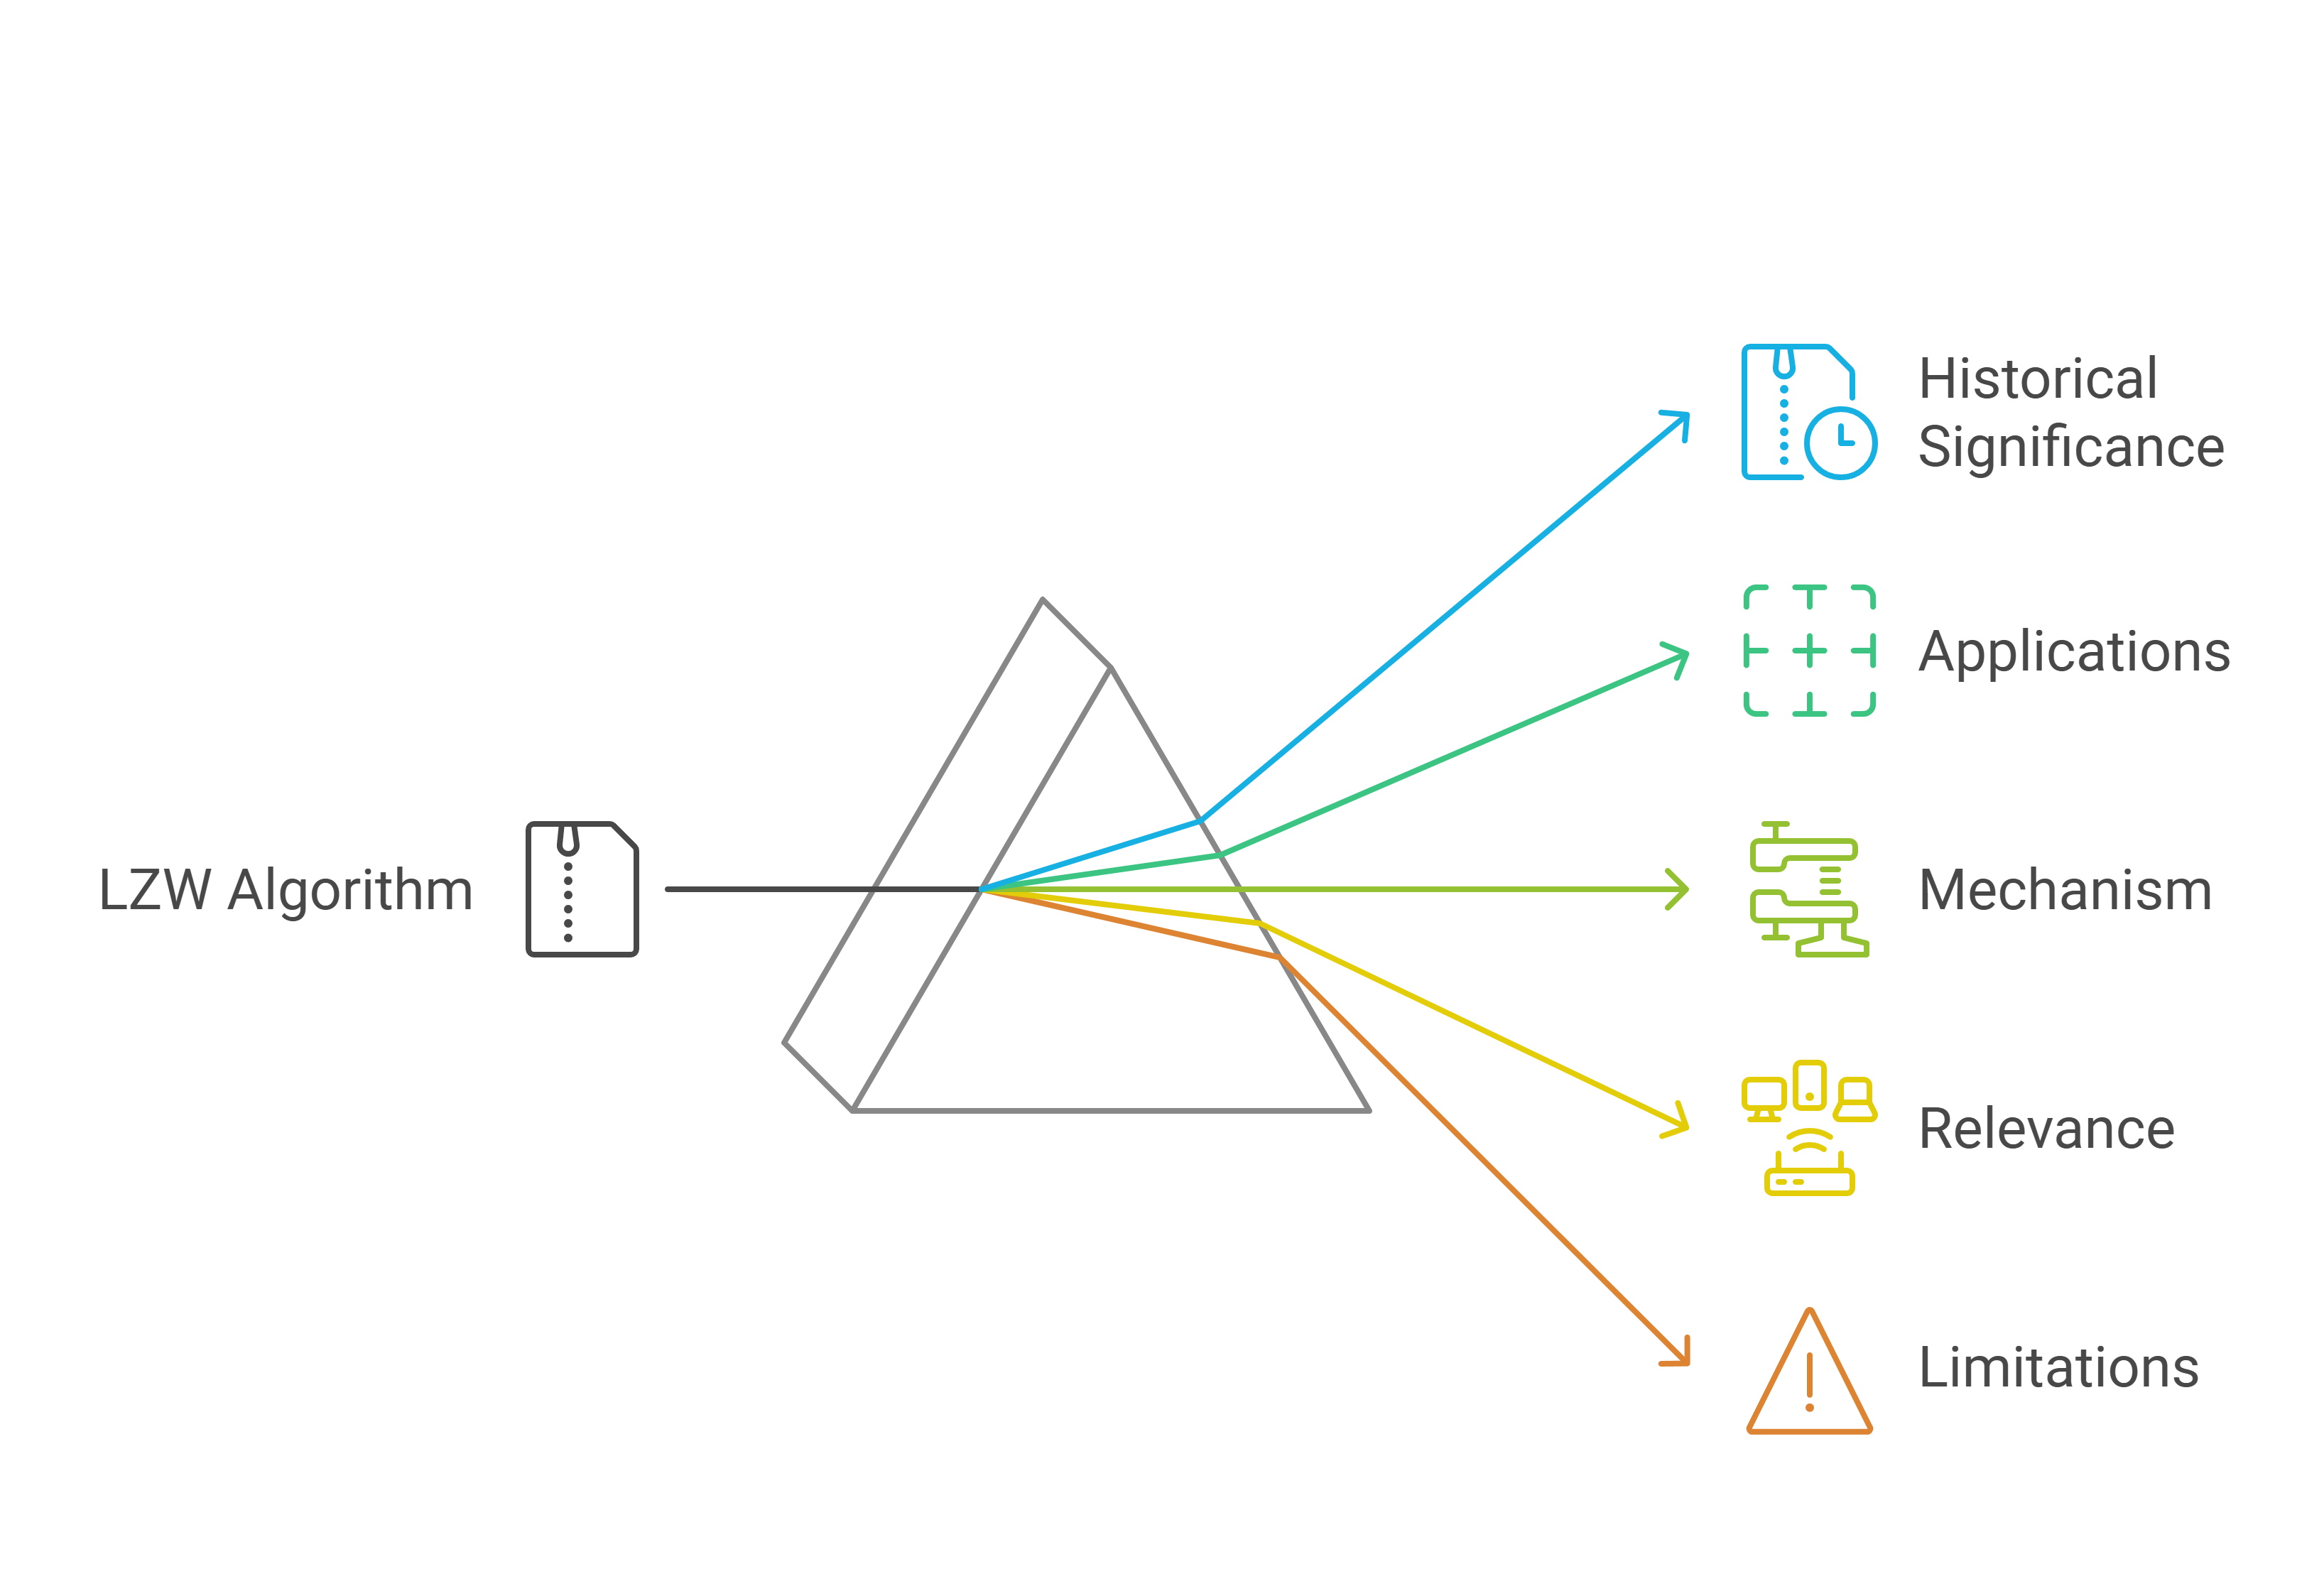
\includegraphics[width=0.7\linewidth]{pic/Conclusion.png}
        \label{fig:enter-label}
    \end{figure}
\end{frame}

% \printbibliography 

\end{document}